\documentclass[14pt,a4paper,oneside]{report}		%lớp văn bản
\usepackage{graphicx}
\graphicspath{ {images/} }
\usepackage[utf8]{vietnam}						%gói ngôn ngữ tiếng Việt
%--
\usepackage{amsfonts}
\usepackage{latexsym, amsmath, amsxtra, amssymb, amscd, amsthm}	%gói ký tự toán
\usepackage{indentfirst}
\usepackage{fancyheadings}
\usepackage{color,colortbl}		%gói màu
\usepackage{graphicx}			%gói hình ảnh 
\usepackage{hyperref}			%gói liên kết link
\usepackage[top=3.5cm, bottom=3.0cm, left=3.5cm, right=2cm] {geometry}
\lhead{Mô hình ngẫu nhiên và ứng dụng}
\rhead{Nhóm 2 - Toán Tin K58}
%//================================= Begin dinh nghia cac goi lenh
\renewcommand{\contentsname}{Mục lục}
\renewcommand{\chaptername}{Chương}
\renewcommand\bibname{Tài liệu tham khảo}
\newcommand{\gach}{\backslash}
\newtheorem{theorem}{Định lý}
%==================================// End dinh nghia cac goi lenh
%//================================== Begin make title
\title{{\bf  BÁO CÁO CUỐI KỲ MÔN MÔ HÌNH NGẪU NHIÊN VÀ ỨNG DỤNG}}
\author{Tác giả: nguoicontraiphonui \hspace*{1cm}Website: http://nguoicontraiphonui.blogspot.com \and \\
Soạn thảo văn bản \LaTeX{} bởi công cụ MikTeX $\&$ TeXmaker\\\\}
\date{{\em \today}}
%==================================// End make  title
\begin{document}
\pagestyle{fancy}	
\Large												%co chu
\maketitle											%make title
\setlength{\baselineskip}{5truept}		%gian dong cho muc luc
\tableofcontents									%tao muc luc
\newpage
\setlength{\baselineskip}{18truept}	%gian dong cho van ban
%//==========================================Begin noi dung bai==
\chapter{Giới thiệu}
Trong ngành khoa học máy tính, học tăng cường (tiếng Anh: reinforcement learning) là một lĩnh vực con của học máy, nghiên cứu cách thức một tác tử (agent) trong một môi trường nên chọn thực hiện các hành động nào để cực đại hóa một khoản thưởng (reward) nào đó về lâu dài. Các thuật toán học tăng cường cố gắng tìm một chiến lược ánh xạ các trạng thái của thế giới tới các hành động mà agent nên chọn trong các trạng thái đó.

Môi trường thường được biểu diễn dưới dạng một quá trình quyết định Markov trạng thái hữu hạn (Markov decision process - MDP), và các thuật toán học tăng cường cho ngữ cảnh này có liên quan nhiều đến các kỹ thuật quy hoạch động. Các xác suất chuyển trạng thái và các xác suất thu lợi trong MDP thường là ngẫu nhiên nhưng lại tĩnh trong quá trình của bài toán (stationary over the course of the problem).

Khác với học có giám sát, trong học tăng cường không có các cặp dữ liệu vào/kết quả đúng, các hành động gần tối ưu cũng không được đánh giá đúng sai một cách tường minh. Hơn nữa, ở đây hoạt động trực tuyến (on-line performance) được quan tâm, trong đó có việc tìm kiếm một sụ cân bằng giữa khám phá (lãnh thổ chưa lập bản đồ) và khai thác (tri thức hiện có). Trong học tăng cường, sự được và mất giữa khám phá và khai thác đã được nghiên cứu chủ yếu qua bài toán multi-armed bandit.
%==============================
\chapter{Phương pháp}
Chương đầu có nội dung như sau

\section{Quá trình quyết định Markov}
Viết vài lời về phần đầu, bao gồm những phần nhỏ như sau
\subsection{{\Large Quá trình Markov}}
viết vào đây....

\subsection{Quá trình Markov có phần thưởng}
viết đây....
\subsection{Quá trình quyết định Markov}
\section{Thuật toán Q-learning}
Q-learning là một kỹ thuật đánh giá hành động nào sẽ được chấp nhận dựa trên một hàm giá trị-hành động xác định giá trị của một trạng thái nào đó và thực hiện một hành động nào đó ở trạng thái đó. 

Chúng ta có một hàm Q với đầu vào là một trạng thái và một hành động,đầu ra là phần thưởng mong đợi của hành động đó (và tất cả các hành động tiếp theo) ở trạng thái đó. Trước khi chúng ta khám phá môi trường, Q cho cùng một giá trị cố định (tùy ý). Nhưng khi chúng ta khám phá môi trường nhiều hơn, Q cho chúng ta một sự ước lượng ngày một tốt hơn về giá trị của một hành động ở trạng thái nào đó. Giá trị của Q được cập nhật liên tục trong quá trình tác tử hành động. 
	Phương trình của Q-learning giải thích tất cả một cách rất độc đáo. Nó cho thấy cách chúng ta cập nhật giá trị của Q dựa trên phần thưởng mà chúng ta nhận được từ môi trường:
\begin{equation}
Q(s_t,a_t) \leftarrow Q(s_t,a_t)+\alpha(r_t+\gamma max_{a}Q(s_{t+1},a) - Q(s_t,a_t)
\end{equation}
Trong đó $Q:S \times A \rightarrow \mathbb{R}$ là hàm đánh giá giá trị chất lương của hành động ứng với trạng thái hiện tại. $r_t$ là phần thưởng đã nhận được ở thời trạng thái hiện tại, $\alpha$ là hệ số học, $\gamma$ là hệ số chiết khấu, và $maxQ(s_{t+1},a_t)$ là giá trị ước tính nhận được trong tương lai. Các biến trên có ảnh hưởng tới thuật toán như sau:
\begin{itemize}
\item \textbf{Hệ số học}: thể hiện cường độ cập nhật giá trị Q. $\alpha$ càng gần 0 thì giá trị Q cập nhật càng chậm, $alpha = 0$ thì tác tử gần như không học được gì, $alpha = 1$ thì có nghĩa là ta thay thế giá trị Q cũ bằng giá trị mới cập nhật, không lưu giữ lại thông tin giá trị cũ. Trong môi trường tất định, $alpha=1$ là tối ưu. Còn trong môi trường ngẫu nhiên, thuật toán chỉ hội tụ khi hệ số học tiến dần tới 0. Trong thực tiễn $\alpha$ thường được chọn là 0.1 tại mọi thời điểm t.
\item \textbf{Hệ số chiết khấu}: xác định tầm ảnh hưởng của phần thưởng trong tương lai. Hệ số chiết khấu càng nhỏ (gần 0) thì tác tử sẽ hầu như chỉ quan tâm tới phần thưởng hiện tại, bỏ qua phần thưởng trong tương lai, ngược lại, hệ số càng gần 1 thì các phần thưởng trong tương lai sẽ được đánh giá cao hơn. Để giá trị của Q hội tụ thì $\gamma$ phải nhỏ hơn 1. Nếu $\gamma$ quá gần 1 cũng sẽ dẫn tới giá trị của Q không ổn định và việc học mất nhiều thời gian. Khi đó việc giảm giá trị $\gamma$ sẽ làm tăng tốc việc học.
\item \textbf{Điều kiện ban đầu $Q_0$} : Do Q-learning là một thuật toán lặp nên việc chọ giá trị khởi tạo có vai trò quan trọng và đòi hỏi kinh nghiệm khi thực hiện. Với giá trị khởi tạo cao, thuật toán có tác dụng khám phá nhiều hơn.
\end{itemize} 

	Thuật toán diễn ra như sau:
\begin{enumerate}
\item Khởi tạo $\gamma$, ma trận phần thưởng R
\item Khởi tạo Q là một ma trận 0
\item Khởi tạo trạng thái ban đầu
\item Lặp các bước sau cho tới khi đạt tới trạng thái mong muốn
\begin{itemize}
\item Chọn một hành động bất kỳ trong số tất cả các hành động có thể theo trạng thái hiện tại
\item Xác định trạng thái tiếp theo
\item Với mỗi hành động có thể, xác định giá trị Q đạt được ứng với trạng thái tiếp theo. Chọn ra hành động cho giá trị Q cao nhất
\item Tính laị giá Q theo công thức 2.1
\item Chuyển trạng thái hiện tại thành trạng thái tiếp theo vừa xác định ở trên và lặp.
\end{itemize}
\end{enumerate}
$\textbf{Xét ví dụ minh họa}$ cho thuật toán Q-learning sau đây: Giả sử tác tử được đặt trong môi trường là một tầng nhà gồm có 5 phòng (đánh số từ 0 tới 4) với các cửa ra vào được bố trí như hình dưới. Không gian bên ngoài tầng nhà được đánh số 5. Từ phòng 1 và phòng 4 có cửa dẫn ra ngoài tầng nhà. Nhiệm vụ của tác tử là tìm cách thoát ra khỏi tầng nhà từ bất kỳ phòng nào, tức là chuyển tới phòng số 5 từ 1 trong các phòng còn lại một cách nhanh nhất.\\
\\
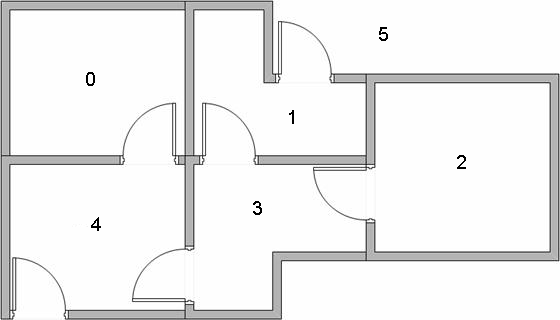
\includegraphics[width=\textwidth,height=\textheight,keepaspectratio]{1.png}
Có thể biểu diễn sơ đồ tòa nhà trên dưới dạng đồ thị có hướng như hình dưới. Mỗi đỉnh của đồ thị biểu diễn một phòng của tầng nhà (hay một trạng thái của tác tử). Nếu có cửa trực tiếp từ phòng này tới phòng kia thì ta có 1 cạnh nối giữa 2 đỉnh tương ứng (biểu diễn hành động của tác tử).\\
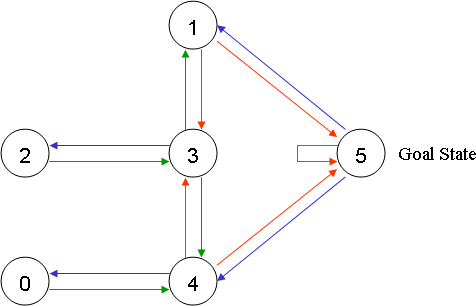
\includegraphics[width=\textwidth,height=\textheight,keepaspectratio]{2.png}
\\
Trọng số của cạnh là phần thưởng cho tác tử khi di chuyển giữa từ phòng này tới phòng kia. Do mục tiêu là thoát khỏi tầng nhà nên hành động trực tiếp thoát ra khỏi tòa nhà được thưởng cao (chẳng hạn được 100 điểm), trong khi những hành động khác không được thưởng (0 điểm) hoặc thậm chí trừ điểm (-1 điểm). Chẳng hạn từ phòng 1 có cửa trực tiếp tới phòng 5 nên cạnh nối đỉnh 1 tới đỉnh 5 có trọng số 100. Từ phòng 1 tới phòng 3 vẫn không thoát được ra ngoài nên cạnh nối từ đỉnh 1 tới đỉnh 3 có trọng số 0, từ phòng 1 không tới trực tiếp được phòng 2 nên cạnh nối từ đỉnh 1 tới đỉnh 2 có trọng số -1. Ta giả sử tác tử bắt đầu từ phòng 2 và cần đi tới phòng 5.\\
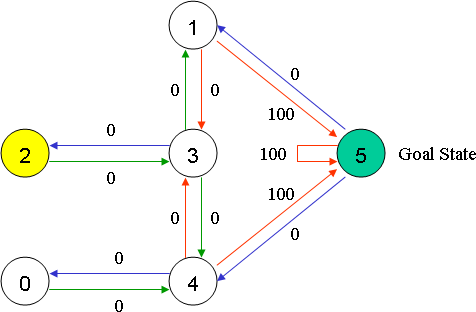
\includegraphics[width=\textwidth,height=\textheight,keepaspectratio]{3.png}
\\
Trong ví dụ này, môi trường là tất định, hệ số học tối ưu $\alpha$ 1. Công thức của thuật toán Q-learning được rút gọn thành:
\begin{center}
$Q(s_t,a_t) = R(s_t,a_t)+\gamma max_aQ(s_{t+1},a_t)$\\
\end{center}
Ta có ma trận phần thưởng trạng thái-hành động tương ứng\\
Khởi tạo ma trận Q là ma trận 0 cỡ $6 \times 6$, hệ số chiết khấu $\gamma = 0.8$\\
$$Q=\begin{bmatrix}
0&0&0&0&0&0\\
0&0&0&0&0&0\\
0&0&0&0&0&0\\
0&0&0&0&0&0\\
0&0&0&0&0&0\\
0&0&0&0&0&0\\
\end{bmatrix}$$\\
Chọn một trạng thái bất kỳ làm trạng thái ban đầu, chẳng hạn  trạng thái 1. Có 2 trạng thái có thể đạt tới đó là trạng thái 3 và trạng thái 5. Chọn ngẫu nhiên, chẳng hạn trạng thái 5. Tính lại Q(1,5):
$$Q(1,5)=R(1,5)+0.8*\text{max}[{Q(5,1);Q(5,4);Q(5,5)}]=100+0.8*0=100$$
Ma trận Q được cập nhật lại:
$$Q=\begin{bmatrix}
0&0&0&0&0&0\\
0&0&0&0&0&100\\
0&0&0&0&0&0\\
0&0&0&0&0&0\\
0&0&0&0&0&0\\
0&0&0&0&0&0\\
\end{bmatrix}$$\\
Như vậy là đã đạt được trạng thái kết thúc. Chúng ta thử một  kịch bản khác bằng việc chọn trạng thái bắt đầu là trạng thái 3. Từ trạng thái này ta chọn một trong các trang thái có thể đạt đến: 1, 2 hoặc 4. Giả sử ta chọn 1. Khi đang ở trạng thái 1. Ta tính lại Q(3,1):
$$Q(3,1)=R(3,1)+0.8*\text{max}[{Q(1,2);Q(1,5)}]=0+0.8*100=80$$
Ma trận Q được cập nhật.
$$Q=\begin{bmatrix}
0&0&0&0&0&0\\
0&0&0&0&0&100\\
0&0&0&0&0&0\\
80&0&0&0&0&0\\
0&0&0&0&0&0\\
0&0&0&0&0&0\\
\end{bmatrix}$$\\
Từ trạng thái 1 ta có thể đến được trạng thái 3 hoặc trạng thái 5. Giả sử ngẫu nhiên ta chọn trạng thái 5. Q(1,5) được tính lại tương tự như trên. Kịch bản này lại kết thúc và ma trận Q thu được:
$$Q=\begin{bmatrix}
0&0&0&0&0&0\\
0&0&0&0&0&100\\
0&0&0&0&0&0\\
0&0&0&0&0&0\\
0&0&0&0&0&0\\
0&0&0&0&0&0\\
\end{bmatrix}$$\\
Cứ như vậy ta đề ra toàn bộ các kịch bản có thể xảy ra. Quá trình trên hội tụ dẫn đến ma trận Q cuối cùng là:
$$Q=\begin{bmatrix}
0&0&0&0&400&0\\
0&0&0&320&0&500\\
0&&0&320&0&0\\
0&400&256&0&400&0\\
320&0&0&320&0&500\\
0&400&0&0&400&500\\
\end{bmatrix}$$\\
Có thể chuẩn hóa ma trận trên bằng cách chia tất cả các phần tử cho phần tử lớn nhất của ma trận. Ta thu được:
$$Q=\begin{bmatrix}
0&0&0&0&80&0\\
0&0&0&64&0&100\\
0&&0&64&0&0\\
0&80&51&0&80&0\\
64&0&0&64&0&100\\
0&80&0&0&80&100\\
\end{bmatrix}$$\\
Từ ma trận trên ta thu được đồ thị mới:\\
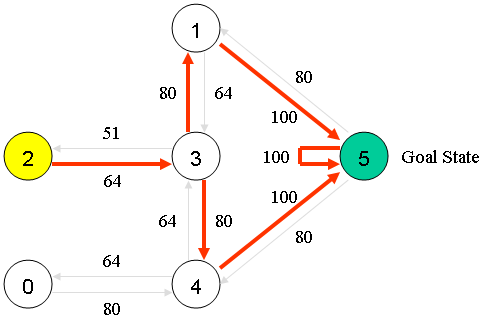
\includegraphics[width=\textwidth,height=\textheight,keepaspectratio]{5.png}
\\
Suy luận từ đồ thị, ta tìm được 1 đường đi từ trạng thái 2 tới trạng thái 5 tối ưu như sau:
\begin{enumerate}
\item Từ trạng thái 2, để Q đạt giá trị max thì di chuyển tới trạng thái 3. 
\item Từ trạng thái 3, để Q đạt max thì di chuyển tới 1 hoặc 4. Chọn di chuyển tới 1.
\item Từ trạng thái 1, để Q đạt max thì di chuyển tới 5.
\item Trạng thái 5 là trạng thái kết thúc. Thuật toán dừng. Ta thu được 1 chiến lược tối ưu: 2-3-1-5
\end{enumerate}

\chapter{Ứng dụng trong thực tế}
\chapter{Kết quả}
\chapter{Tổng kết và bàn luận}
%============================
%Tài liệu tham khảo
\begin{thebibliography}{12}
\addcontentsline{toc}{chapter}{\quad\  \bf Tài liệu tham khảo}
\bibitem{1}Họ và tên tác giả, năm, {\it Tên sách} NXB.
\bibitem{2}Họ và tên tác giả, năm, {\it Tên sách} NXB.
\bibitem{3}Họ và tên tác giả, năm, {\it Tên sách} NXB.
\bibitem{4}Họ và tên tác giả, năm, {\it Tên sách} NXB.
\bibitem{5}Họ và tên tác giả, năm, {\it Tên sách} NXB.
\end{thebibliography}

\end{document}
